\chapter{Background, Motivation, and Overview}
\label{chap:intro}

%=====================================================================================================
\section{Introduction}
\label{intro}
%About 5 pages answering questions 1 and 2 above, along with describing the broad research area. This section provides the reader with enough information to understand and appreciate the thesis statement. This includes giving the motivation for the research, defining terms and formulating the problem. Often, subsections labeled ``Background'' and ''Motivation'' will be included in this section. This section typically provides answers to the questions ``What problem do you want to solve'' and ''Who cares about this problem and why?'' The Background subsection could contain the discussion about the broader research area.

%===================================================
\subsection{Problem Motivation}
\label{motivation}

Because of rapid advancement in technology, more and more Artificial Intelligence (AI) and robotics systems are appearing in various aspects of people's lives. For example, there are systems that assist humans to schedule limousine services~\cite{Chun2010Limousine}, to evaluate and control the damage of an oil spill\footnote{http://spectrum.ieee.org/robotics/industrial-robots/the-gulf-spills-lessons-for-robotics}, to support search and rescue missions~\cite{Casper2003Human,Lin2010Supporting}, and to provide treatment to children with autism~\cite{Robins2009From}. Such abundant and rapidly growing applications increase the set of possible interactions between human users and autonomous systems. The humans in such interactions are not likely the designers of the autonomous systems, but these humans must still manage the autonomy.

Although AI and robotics systems have grown to be able to handle increasingly complex tasks in uncertain environments, human assistance and supervision are often needed~\cite{Bainbridge1983Ironies}. Even for fully autonomous systems, human input can potentially improve the system's performance and safety. Human experts can use domain-specific knowledge to assist an AI/robotics system when it deals with changing environments, uncertainty, and case-specific scenarios. Therefore, it is necessary to design tools and interfaces that enable human users working with an AI/robotics system to manage the autonomous behaviors of the system efficiently and effectively; such tools can improve task performance and the experience of a human partner in human-automation interaction. 

However, human users often do not understand how the internal mechanisms of an autonomous system work especially when the system is complicated or when complex algorithms are involved. Instead, humans must rely on their own mental models of the system during operation~\cite{Moray1999Mental}. Supporting human interaction requires a design approach that lets users understand how autonomous behaviors can be influenced without getting deeply into how autonomy really works. This requirement makes designing for autonomy management especially challenging.

%===================================================
\subsection{General Solution Approach}

We propose that autonomy management tools should let users hierarchically manage information provided to an AI/robotics system. Good information management tools should allow users to influence the autonomous behaviors of the system at multiple scales without the need for tedious direct/manual control. This dissertation presents autonomous algorithms/components and autonomy management tools/interfaces designed at different scales and show that this approach improves the performance of the human-automation team and the experience of the human-automation interaction.

The term ``information'' here covers a wide range of things including \textit{knowledge of the environment} (including other humans, equipment, and changes in the physical surroundings), \textit{knowledge of the task} at hand (including processes, procedures, rules, past experiences, etc.), and \textit{interactions among various entities} (task, environment, human, and the system). In theory, an AI/robotics system can obtain, process, and analyze information in order to complete the desired tasks. In practice, however, the system often has limited sensing and reasoning capabilities, and there is useful information the system is either not capable of obtaining or not able to understand/process. Such information can even be produced by the system itself. Often, the human users of such systems have much better ``information sensing'' capabilities. These capabilities allow humans to obtain information from their own resources such as past experiences, domain-specific training, external communications (with team members, external systems, etc.), or even the AI/robotics system itself. The human user is also capable of ``digesting'' various information and then feeding the ``filtered'' information to the system in forms the system can understand. In a sense, the human user acts as an ``intelligent sensor'' for the system. At the same time, by deciding what information to provide to the system, the human user has a way of influencing the system's autonomous behaviors without the need for tedious manual control.

%\begin{figure}
%\centering
%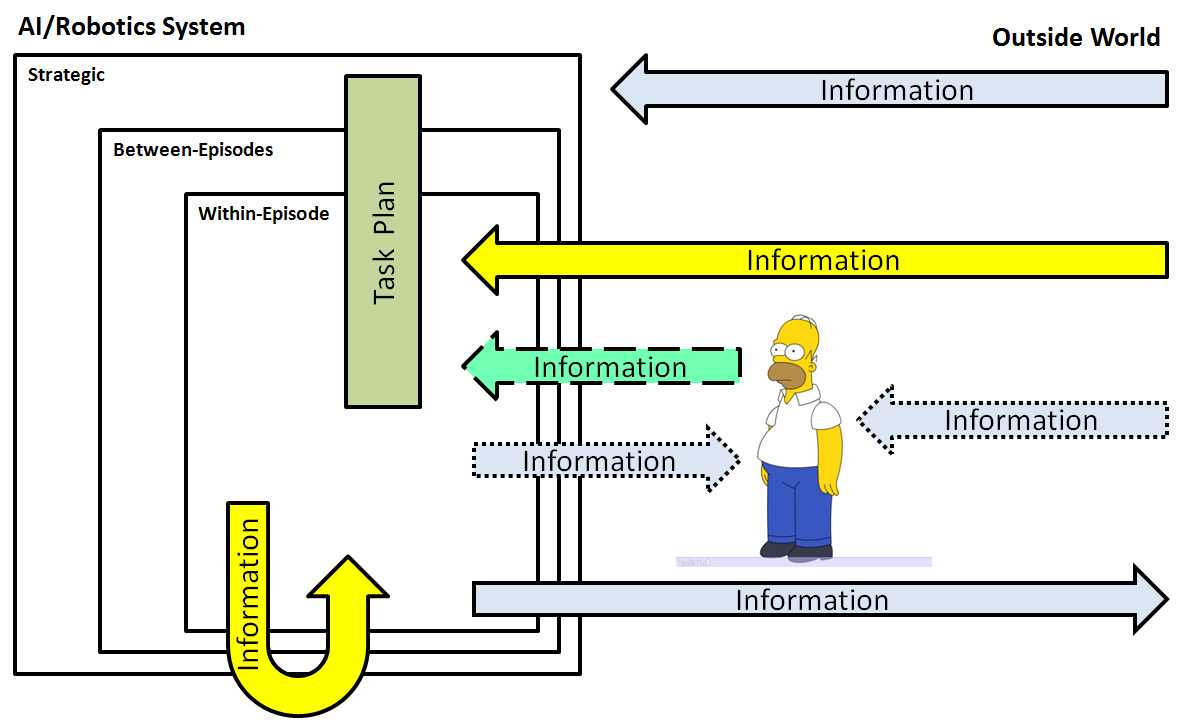
\includegraphics[width=4.5in]{System.png}
%\caption{Diagram showing relationship between the human user and the AI/robotics System with respect to information management.}
%\label{system}
%\end{figure}

%Figure~\ref{system} shows a diagram of the relationship between the human user and the AI/robotics system. The system must be capable of receiving the outside information at different scales (solid yellow arrow at the top). The system has some degree of sensor-processing, so it naturally uses internal information to make decisions (solid yellow arrow at the bottom). The human can sense and process information the system is not capable of handling. Such information can be directly from the outside world (dotted blue arrow on the right) or perceived through the system's sensors (dotted blue arrow on the left). The human processes the information and feeds filtered information to the system, in forms the system can understand (dashed green arrow), in order to influence the system's autonomous behaviors.

\begin{figure}
\centering
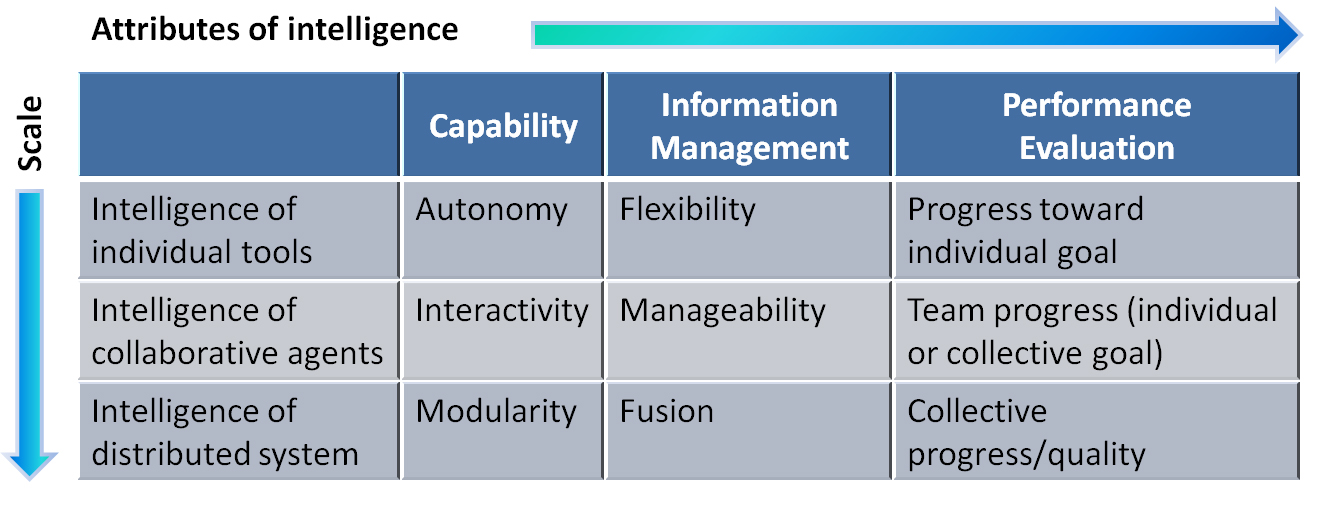
\includegraphics[width=6in]{IntegrationChallenges.JPG}
\caption{Autonomy integration challenges defined along two dimensions. Horizontal dimension: attributes of intelligence. Vertical dimension: scale.}
\label{challenges}
\end{figure}

In an overall integrated intelligent system, autonomy typically exists as component tools with the goal to offload portions of responsibility to autonomous algorithms. Figure~\ref{challenges} lists some key elements of the autonomy integration challenges we identified in~\cite{Lin2010Supporting} along two dimensions: \textit{attributes of an intelligent system} (capability, information management, performance evaluation) and \textit{scale} (individual versus group, expanded to include a new row for intelligence of collaborative agents). This table provides guidelines on what attributes should be designed into an autonomous component when it is part of a human-automation collaboration team and a much larger distributed intelligent system. As an individual tool, the autonomous component needs to be able to perform certain tasks (\textbf{autonomy}). It should be able to work with different scenarios and can be interrupted, temporarily aborted, and possibly resumed later depending on information available to the operator (\textbf{flexibility}). If a human agent is in a collaborative team with the autonomous agent for the same task, the autonomous component must provide ways of interaction (\textbf{interactivity}) so the human can manage how the autonomous component works based on information only the human can interpretate (\textbf{manageability}). It is different from flexibility because the human agent can actually influence the behaviors of the autonomous compoment through information management. Then in order to integrate the autonomous component into the overall distributed system, the autonomous component has to be modular so it is easy for human operators to share responsibilities or (partially) take on responsibilites of different roles (\textbf{modularity}). And information from various sources (including information output from autonomous components) need to be combined and presented intelligently in an efficient way to relavant users (\textbf{fusion}). Autonomous components presented in this dessertation all contain these important attributes. Specifically, we design our autonomous components with the capability to interact with information representations so the human agent can manage autonomy by hierarchically managing information. 

Good autonomy management tools will only let users manage information that allow them to develop a clear causal relationship between information management actions and the changes of the system's autonomous behaviors. Examples of such information include what data set to use to train the system and which tasks deserve more attention. Such causal relationships make developing correct mental models of the system easier leading to improved task performance. 

Information can be managed at different temporal scales. 
%We use the term ``resolution'' to describe the levels of details involved. Working at a high resolution is like working with individual pixels in an image to achieve fine precision, whereas working at a low resolution is more like working on object attributes such as shapes or shadings that are viewed better when one takes a step back from the image and ignores the fine details. Similarly, managing autonomy at a high resolution involves managing the actions of the AI/robotics system in fine details (e.g., managing waypoints a UAV should follow), and at a low resolution autonomy management might deal with strategic planning following generate trend (e.g., predicting and identifying high priority areas in a WiSAR operation).
We propose a general hierarchical framework that focuses on the following three scales: \textbf{Strategic}, \textbf{Between-Episodes}, and \textbf{Within-Episode}\footnote{The term ``episode'' we use is similar to the one Russell and Norvig define in Chapter 2 of~\cite{Russell2009Artificial} when they discussed episodic vs. sequential task environments. Our definition is more relaxed to include cases where actions taken in previous episodes might impact the current episode with respect to task objectives, but each episode is still by itself a separate and self-contained unit.}. 

When an AI/robotics system is given a task, the system can generate an initial plan based on its model(s) of how this kind of task is generally performed. This step is planning at the \textbf{Strategic} scale. Since the same task can be performed in different case scenarios (such as different environments, constraints, or phases of the operation), case-specific attributes and requirements need to be evaluated, and the initial plan needs to be tailored to the specific case. This step is planning at the \textbf{Between-Episodes} scale. During execution of the task, the plan is carried out, but as new information becomes available or when the environment changes due to uncertainty, the plan can be modified in real time to achieve better task performance. This step is planning at the \textbf{Within-Episode} scale. If the user of the system can manage information provided to the system by selecting what information to provide at what scale, he/she can change the system plan at different scales and indirectly influence the autonomous behaviors of the system.

To evaluate the usefulness of the proposed autonomy management approach, we apply it to the application domain of using an Unmanned Aerial Vehicle (UAV) to support Wilderness Search and Rescue (WiSAR).

%===================================================
\subsection{Application Domain}

A small camera-equipped UAV can quickly and cheaply provide aerial imagery of a wilderness search area, especially hard-to-reach areas~\cite{Goodrich2008Supporting}. The MAGICC lab, the HCMI lab, and the Computer Vision Lab at BYU have been researching UAV technologies for several years and made great progress in UAV path-planning control, user interface design, and computer vision~\cite{Lin2010Supporting}. Figure~\ref{SystemComponents} shows the various components developed by the research group. This dissertation focuses on the three highlighted components that are related to the UAV path planning problem.

\begin{figure}
\centering
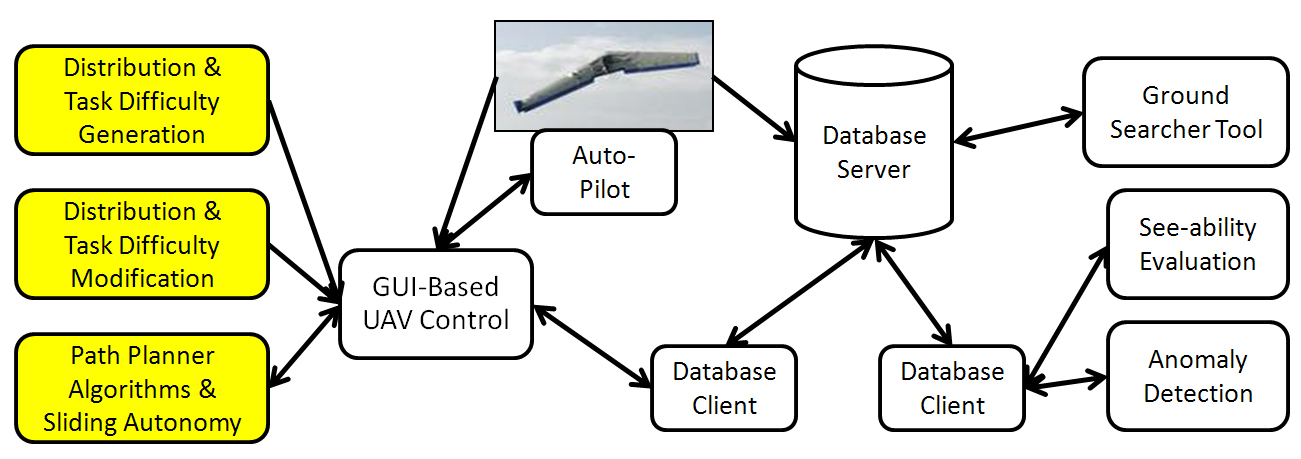
\includegraphics[width=6in]{UAVWiSARComponents.JPG}
\caption{Various components of the overall intelligent system (a distributed system) of using a UAV to support Wilderness Search and Rescue. The three highlighted components are related to UAV path planning.}
\label{SystemComponents}
\end{figure}

Past UAV field trials indicate that real WiSAR searchers like not having to worry about keeping the UAV in the air or setting waypoints manually. Autonomy that offloads or complements some search work is useful, but searchers also need to be able to manage where to send the UAV as new evidence is gathered or hard-to-reach areas are identified. Ideally, searchers need not understand the statistical models or complex algorithms used by the UAV. Rather, searchers should manage autonomy by managing information provided to the UAV system at different scales. We focus on two important representations of information: a \textit{probability distribution map} and a \textit{task-difficulty map} as shown in Figure~\ref{Scales}.

\begin{figure}
\centering
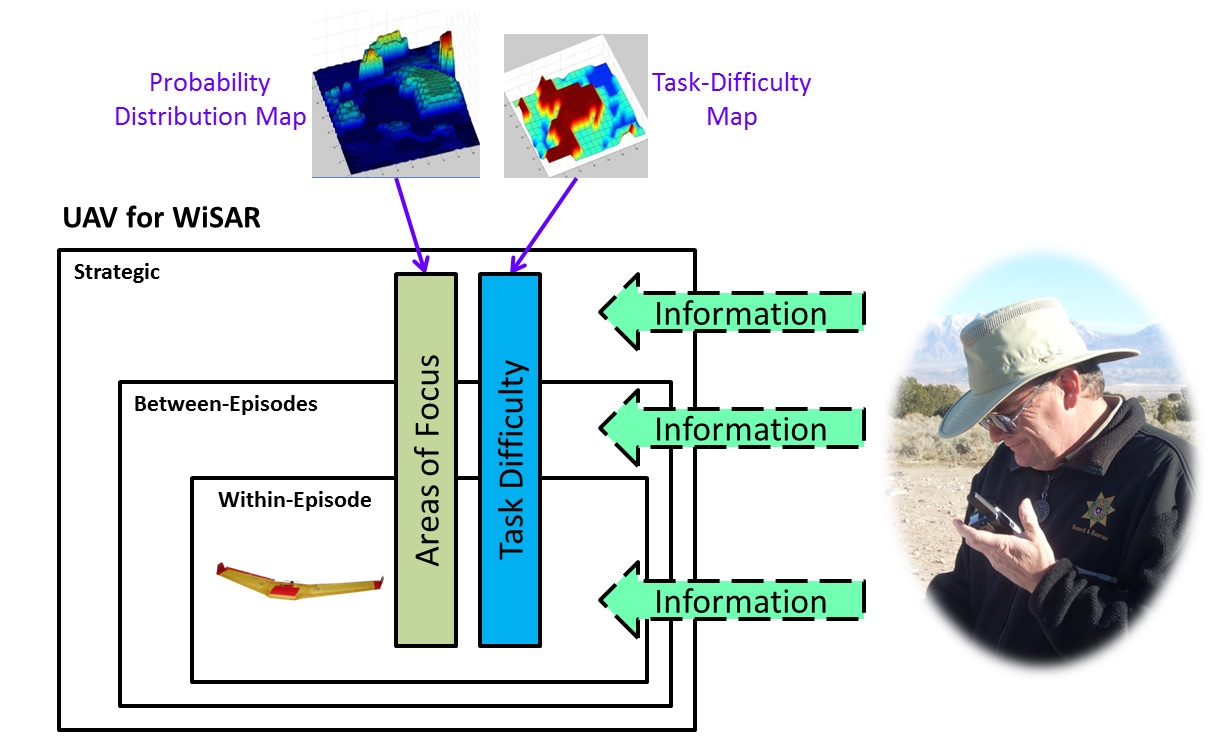
\includegraphics[width=6in]{scales.JPG}
\caption{WiSAR searchers can manage autonomy by managing a \textit{probability distribution map} and a \textit{task-difficulty map} at different scales of the sytem.}
\label{Scales}
\end{figure}

Following the guidelines in Figure~\ref{challenges}, we developed autonomous components/algorithms and mangement tools/interfaces that meet the challenges of an integrated system and also support collaboration between a human agent and an autonomous agent at different scales. At  the \textbf{Strategic} scale, we developed the \textbf{DistCreate} and \textbf{DiffCreate} components. \textbf{DistCreate} uses a Bayesian model to predict the probability distribution of the missing person's likely location, using terrain features of the search area and past human behavior data in the form of GPS track logs. Domain users can affect the model-generated probability distribution by changing prior beliefs parameters and by determining what human behavior data (data for selected regions, season, or missing person characteristics) to feed to the model. \textbf{DifCreate} is a simple tool that automatically generates a task-difficulty map, a representation marking areas with low probability of detection, based on vegetation coverage Lansat data from USGS satelite imagery servers\footnote{http://www.usgs.gov/pubprod/}. At the \textbf{Between-Episodes} scale, we developed two management tools: \textbf{DistEdit}, a tool that lets the user modify the probability distribution to specify areas of focus with simple gestures, and \textbf{DiffEdit}, a tool that lets the user use scribbles to modify the task-difficulty map. At the \textbf{Within-Episode} scale, we developed a bunch of path planning algorithms that support partial detection and real-time feedback. We also present a \textbf{SlidingAutonomy} interface that lets a human agent manage UAV autonomy along two dimensions: a temporal dimension deciding how much time is granted to a UAV for each path segment, and a spatial dimension determining what  constraints (path segment ending points) to impose to the path planning task.


%=====================================================================================================
\section{Related Work}
\label{related}
%About 2 pages answering question 3 above. This section contains a survey of the literature directly related to the problem you are trying to solve (i.e., thesis statement) and should demonstrate to your readers that you understand the context of your work. This is a place for you to position your contribution to your specific research area relative to other work that has been done, and to state how your work builds on the previous work. In most cases there will be only a small overlap between the papers discussed in this section and the papers related to the broader research area. This section answers the question ``What have others done to solve the problem and why is this inadequate?''

In their in-depth survey paper~\cite{Goodrich2007HRISurvey}, Goodrich and Schultz define the HRI problem as ``understanding and shaping the interactions between one or more humans and one or more robots.'' They also specified robot-assisted search and rescue as a key area for HRI research. In this section we first present related work in the general research area, then discuss related research more specific to the domains of using UAVs to support Wilderness Search and Rescue.

%===================================================
\subsection{General Research Area}

When humans and robots work together as a team, balancing responsibilities between human and automation becomes a difficult challenge. Drucker defines automation as a ``concept of the organization of work~\cite{Drucker2006Practice}.'' In their 1978 seminal paper~\cite{Sheridan1978Human}, Sheridan and Verplank propose the idea of a \textit{Level of Autonomy} spectrum. At one end of the spectrum is full teleoperation and at the other is full autonomy. In the middle of this spectrum, the robot could suggest actions to humans or make decisions before informing humans. Parasuraman et al.\ \cite{Parasuraman2000Model} extended this one-dimensional spectrum to four different broad functions: information acquisition, analysis, decision selection, and action implementation. 

In~\cite{Sheridan1992Telerobotics} Sheridan proposes \textit{Supervisory Control}, in which a human divides the task into a sequence of subtasks that the robot is capable of performing, and the human then provides guidance when the autonomous system cannot solve a problem on its own. In contrast to the top-down philosophy of supervisory control, a \textit{Mixed-initiative} approach advocates the idea of dynamically shifting tasks when necessary~\cite{Hearst1999Mixed}. \textit{Collaborative Control}, which can be thought of as an instance of mixed-initiative interaction, is a robot-centric model; instead of the human always being in-charge, the robot is treated as a peer and can make requests to humans through dialogs~\cite{Fong1999Collaborative}. \textit{Adjustable Autonomy}~\cite{Dorais2001Designing} (also referred to as \textit{Sliding Autonomy}~\cite{Dias2008SlidingAutonomy} or \textit{Adaptive Automation}~\cite{Rouse1988Adaptive}) is another type of mixed-initiative interaction, one that enables the human-automation team to dynamically and adaptively allocate functions and tasks among team members. Bradshaw et al.\ \cite{Bradshaw2004Dimensions} propose two dimensions of Adjustable Autonomy (descriptive  and prescriptive) to address the two senses of autonomy (self-sufficiency and self-directedness) and discuss how permissions, obligations, possibilities, and capabilities can be adjusted. Bradshaw et al.\ \cite{Bradshaw2013Seven} also summarized some widespread misconceptions on autonomy and listed seven deadly myths of ``autonomous systems.''

Scholtz defines in~\cite{Steinfeld2006Common} four roles for a human agent in human-robot interaction: supervisor, operator, mechanic, peer, and bystander. Goodrich and Schultz suggests two more roles: mentor and information consumer~\cite{Goodrich2007HRISurvey}. Then Humphrey and Adams adds another role, abstract supervisor~\cite{Humphrey2009Information}. With our information management approach, users can act as ``intelligent sensors'' and manage what information to feed the system at different scales. Therefore, the human is taking on a smart ``information sensor'' role in HRI. The idea of using humans as sensors is not new. For example, Kaber et al.\ advocate using humans as active information processors in complex systems to support situation awareness and effective performance~\cite{Kaber2001Design}. Bourgault et al.\ include humans as augmented sensor nodes in a wilderness search task~\cite{Bourgault2008AugmentedNodes}. Other researchers have experimented with management at different resolution. Dias et al.\ \cite{Dias2008SlidingAutonomy} propose enabling interactions at different levels of granularity. However, using information as a control mechanism to manage autonomy at the three distinctive scales we identified is different from previously published approaches.

One component of our proposed solution, the \textbf{SlidingAutonomy} interface, falls under the category of \textit{Adjustable Autonomy}. Dorais et al.\ \cite{Dorais1998AdjustableAutonomy} discuss a framework for human-centered autonomous systems for a manned Mars mission. The system enables users to interact with these systems at an appropriate level of control but minimize the necessity for such interaction. Bradshaw et al.\ discuss principles and pitfalls of adjustable autonomy and human-centered teamwork, and then present study results on so-called ``work practice modeling'' and human-agent collaboration in space applications~\cite{Bradshaw2003AdjustableAutonomy}. In~\cite{Kaber2005Adaptive} Kaber et al.\ describe an experiment simulating an air traffic control task where manual control was compared to Adaptive Automation (AA). Results suggest that humans perform better with AA applied to sensory and psychomotor information-processing functions than with AA applied to cognitive functions; these results also suggest that AA is superior to completely manual control. Brookshire et al.\ present preliminary results for applying sliding autonomy to a team of robots performing coordinated assembling work to help the system recover from unexpected errors and to thereby increase system efficiency~\cite{Brookshire2004Preliminary}. Dias et al.\ identified six key capabilities that are essential for overcoming challenges in enabling sliding autonomy in peer-to-peer human-robot teams~\cite{Dias2008SlidingAutonomy}.

Human is an integral part of the human-automation team. When working with automation, the human often takes on the supervisor role. Bainbridge points out that automation requires the human operator to take additional management responsibilities~\cite{Bainbridge1983Ironies}, and Sartar identified in~\cite{Sarter1998Making} two automation management policies: \textit{management by consent} and \textit{management by exception}, defining whether the human always retain authority or can the system take initiative. For complex automations, the human tends to rely on his/her \textit{mental models} (defined by Norman in~\cite{Norman1983Some}) to manage the system. Moray~\cite{Moray1999Mental} provides a good summary of how mental models are used and proposes that mental models ``allow operators to think about causal structures and functions in systems which they must control....'' Goodrich and Boer present a case study of Adaptive Cruise Control design and explain how an automobile driver can switch among multiple mental models and use different management strategies~\cite{Goodrich2002Multiple, Goodrich2003Model}. Lee and See propose that because people respond to technology socially, trust guides reliance when unanticipated situations make it impractical or impossible to understand automation~\cite{Lee2004Trust}. Hoffman et al.\ \cite{Hoffman2013Trust} suggests ``active exploration for trusting''(AET) and hope this approach can promote both trust ``calibration'' and appropriate reliance. Moray also points out that the operator's internal model of the environmental and task dynamics can affect how the operator samples information from the environment, and display interfaces should be designed to attract the right amount of attention~\cite{Moray1990Designing}. In~\cite{Vicente1997Should} Vicente suggests to follow the ecological approach~\cite{Rasmussen1994Cognitive} and design interfaces compatible with the actual constraints of the environment so the operator's understanding corresponds to the actual behavior of the system. Our information management approach and proposed tools are compatible with these principles because they allow a user to infer causal relationship between user actions and autonomous behavior changes. The user interface designs enable the user to develop mental models of the system that match how the system truly works and thereby improve the human-automation interaction experience.

Properly evaluate human-robot interaction has always been a challenging problem due to the diversity of team setups, environmental contexts, and tasks involved. Many metrics have been proposed in the literature. Crandall and Goodrich proposed a metric called Neglect Time to measure interaction efficiency~\cite{Crandall2002Principles}. Together with Neglect Time, Olsen and Goodrich later added Task Effectiveness, Robot Attention Demand, Fan Out, and Interaction Effort to the list of Metrics~\cite{Olsen2003Metrics}. Steinfeld and et al.\ suggest some common metrics for standardizing task-oriented human-robot interaction~\cite{Steinfeld2006Common}. In~\cite{Olsen2007Evaluating}, Olsen presents a set of criteria for evaluating new UI systems. Crandall and Cummings propose in~\cite{Crandall2007Ddentifying} a set of metric classes that can predict how many robots should be in the team and the system effectiveness for single-operator controlling multiple robots. We follow guidelines provided in these papers to validate our proposed solution.

%===================================================
\subsection{Supporting Wilderness Search and Rescue with a UAV}

The goal of our research is to support fielded missions in the spirit of Murphy's work~\cite{Casper2003Human}. UAV technology has emerged as a promising tool in supporting WiSAR~\cite{Murphy2008Cooperative,Bourgault2003Coordinated}. In~\cite{Bourgault2006Optimal, Bourgault2004Coordinated} Bourgault et al.\ describe how to use a Bayesian model to create paths for a single UAV or multiple coordinated UAVs to maximize the amount of probability accumulated by the UAV sensors. In~\cite{Bourgault2008AugmentedNodes} they also include scalable collaborative human systems as augmented sensor nodes and created paths for human ground searchers.

The BYU WiSAR research group has developed a variety of technologies to support Wilderness Search and Rescue with small fixed-wing UAVs~\cite{Beard2005Autonomous, Goodrich2008Supporting, Goodrich2009Towards, Lin2010Supporting}. The UAV system has many autonomous capabilities. The UAV's autopilot can stabilize the UAV during flight, support waypoint following and auto launch/land modes, and provide gimbaled camera control. Simple flight patterns and safety features are available when combining the autopilot with UAV control interfaces~\cite{Beard2005Autonomous, Lin2010Supporting}. These basic UAV capabilities have been greatly extended to provide better WiSAR support: A Bayesian model was developed by Lin and Goodrich~\cite{Lin2010Bayesian} that uses terrain features to predict the likely locations of finding a lost person. Then, Generalized Contour Search~\cite{Goodrich2008Supporting} and Intelligent Path Planning~\cite{Lin2009UAV,Niedfeldt2010integrated} algorithms have been used to automatically generate flight paths for the UAV. A real-time temporally local mosaic technique~\cite{Morse2008Application} has been used to ``stitch'' multiple video frames to provide increased opportunity for detection and increased sense of relative spatial relationships for video analyst. Anomaly detection algorithms~\cite{Thornton2011Unusual} are also available that can mark objects with unnatural colors and alert the video analyst. A metric named ``see-ability''~\cite{Morse2010UAV} was also developed to understand search-related video quality and to index geo-tagged video frames. 

Many path planning algorithms in the literature address obstacle avoidance while planning a path to reach a destination using A*~\cite{Quigley2005Towards}, LRTA*~\cite{Howlett2006Learning}, D*~\cite{Stentz1997Optimal}, Voroni diagrams~\cite{Bortoff2000Path,Beard2005Autonomous}, or probability roadmaps and rapidly-exploring random tree (RRTs)~\cite{Pettersson2006Probabilistic}. Hierarchical heuristics approaches were also developed, such as Hierarchical A* (HA*) by Holte et al.\ ~\cite{Holte1996Hierarchical}, hierarchical task-based real-time path planning by Naveed et al.\ ~\cite{Meuleau2007Hierarchical}, and Hierarchical-AO* (HiAO*) by Meuleau and Brafman~\cite{Naveed2010Hierarchical}. The algorithms we present solve a different path planning problem by generating paths that make efficient use of the limited travel time and maximizing the probability of finding the missing person. This is similar to the Vehicle Routing Problem~\cite{Laporte1992Vehicle} and the Orienteering Problem (OP)~\cite{Golden1987Orienteering}, which is a variation of the Traveling Salesman Problem (TSP) (with names such as Prize-Collecting TSP (PCTSP)~\cite{Gutin2002Traveling} or TSP with profits~\cite{Feillet2005Traveling}), and is known to be NP-Hard~\cite{Sokkappa1990Cost}. Vansteenwegen et al.\ \cite{Vansteenwegen2011Orienteering} gives a good survey on the topic of OP, and listed various approaches such as exact methods~\cite{Laporte1990Selective,Fischetti1998Solving,Ramesh1992Optimal}, approximation heuristic approaches~\cite{Mittenthal1992Insert,Chao1996Fast,Ramesh1992Optimal}, Genetic Algorithm approach~\cite{Tasgetiren2000Genetic}, and Ant Colony Optimization approach~\cite{Liang2006Ant}. These algorithms work well with OP problems of small number of nodes (21--100 nodes). However, our path planning problem requires up to 1800 nodes with added challenges of repeated visits and partial detection.
 
In order to intelligently plan paths for a UAV, it is necessary to understand missing person behaviors and generate a probability distribution of likely places to find the missing person. Many researchers analyzed past WiSAR cases in order to understand missing person behaviors~\cite{Setnicka1980Wilderness,Hill1998Lost,Syrotuck2000Analysis,Heth1998Characteristics,Koester2008Lost}.~\cite{Syrotuck2000Introduction} describes how to use mathematical models to calculate the probability of detection, probability of area and probability of success. He also describes an example search mission. Researchers also looked at systematically utilizing GIS (Geographic Information System) information for search and rescue applications~\cite{Ferguson2008GIS,Soylemez2006Utility}.

Due to factors such as lighting conditions, dense vegetation, or human observer cognitive workload, even when sensor footprint covers the location of the missing person, probability of detection can be less than 1. In the 1950's, Koopman discussed the uncertainties in the act of detecting hostile submarines with radars and proposed a concept called the instantaneous probability of detection by one glimpse~\cite{Koopman1956Theory}. He presented simple search algorithms and demonstrated how search effort should be distributed given a prior probability distribution of the target and known law of detection when only a limited total amount of search effort (or time) is available~\cite{Koopman1957Theory}. Stone~\cite{Stone1975Theory} presents various search plans with partial detection models using Lagrange multipliers and maximization of Lagrangians in finding stationary target in very basic search problems when no false targets are present. Washburn~\cite{Washburn1981Search} discusses how to construct optimal search paths for different search problems. The author also developed detection models based on radar/sonar and expanded the fundamentals of search theory to include moving targets. More recent work includes~\cite{Niedfeldt2010integrated} where Niedfeldt et al.\ present a UAV path planning algorithm that utilizes probability of detection and maximizes the probability of identifying an object using a N-step lookahead method, and~\cite{Ryan2010particle} where Ryan and Hedrick developed a control formulation for a fixed-wing UAV that minimizes the entropy of an estimate distribution over a receding horizon for searching a moving target over a fixed time horizon. Stone et al.\ used posterior probability maps and successfully located the wreckage of Air France Flight 447~\cite{Stone2011Search}. Metrics such as Koopman's instantaneous probability of detection by one glimpse~\cite{Koopman1956Theory}, ``seeability'' proposed by Morse et al.\ \cite{Morse2010UAV}, and terrain and vegetation information obtained from USGS~\cite{Lin2010Bayesian} can be used to build a task-difficulty map representing probability of detection in different search subregions.

The UAV technology is an intelligent system with the integration of many component autonomous algorithms and user interfaces. Integration at this level requires tremendous effort. Salas and Fiore~\shortcite{Salas2004Team} provide great insights on challenges across people and machines, and across time and space in distributed teams. Sycara and Lewis~\shortcite{Sycara2002Integrating} also asked the questions: 1) can a software agent perform the task? and 2) can the agent's assistance contribute toward team performance? Tso et al.\ ~\shortcite{Tso1999Multi} identified that integrating a UAV into the search task creates at least two roles: a pilot that controls the UAV and a sensor operator that analyzes the sensor outputs, and lessons from other search-related domains~\cite{Drury2003Awareness} show that multiple roles are required and these roles can be supported by autonomy algorithms and user interface technologies. These findings motivate and guide our research in developing UAV technology to support WiSAR operations.

%=====================================================================================================
\section{Thesis Statement}
\label{thesis}
%1 to 2 sentences stating what is to be demonstrated in your dissertation. A clear and concise statement of what is to be demonstrated or developed in your dissertation work. A good thesis statement makes a specific claim that your readers care about. Ideally, your introduction will give your readers the background they need to understand your thesis statement and to conclude that it matters.

Designing autonomous components and autonomy management tools that let users manage information provided to an intelligent system at different scales allow users to influence the autonomous behaviors of the system without the need for tedious direct/manual control. This approach improves both the human's experience during the human-automation interaction and the performance of the human-automation team.

%=====================================================================================================
\section{Project Description}
\label{project}

%About 5 pages answering question 4 above. This section describes your preliminary ideas on how you might solve the problem and the anticipated contribution your research will make to the field of Computer Science. This section should convince your committee that you are qualified to pursue the research and have high potential to eventually be able to objectively and convincingly defend your thesis statement. This section answers the question ``What is your proposed solution to this problem?''

We propose a new autonomy management approach that lets users manage the autonomous behaviors of an AI/robotics system by hierarchically managing information at different scales. In this section, we describe how we apply the approach to using a UAV to support WiSAR operations, and relate chapters of the dissertation to components of the hierarchical approach. At each scale, we briefly discuss what autonomous components and autonomy mangement tools we developed, what kind of information the user can manage, and direct readers to the related chapter for more details.
 
%===================================================
\subsection{Solution Overview}

%In this section we show how we apply the proposed autonomy management approach to using a UAV to support WiSAR operations. We describe the designs and requirements of autonomy management tools at each scale and resolution and how they enable users to manage the autonomy behaviors of the UAV system by managing information.

\begin{figure}
\centering
\begin{tabular}{cc}
	\begin{minipage}{0.45\textwidth}
	\centering
	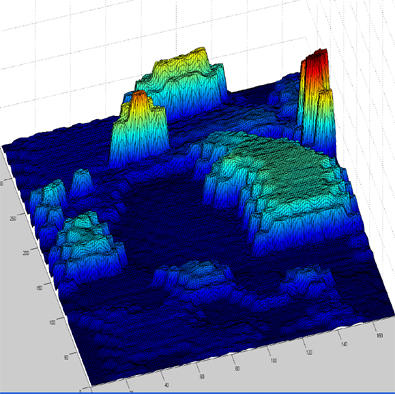
\includegraphics[width=2.8in]{3DMapDist.jpg}
	\caption{An example probability distribution map generated by a Bayesian model.}
	\label{3DMapDist}
	\end{minipage}
&
	\begin{minipage}{0.45\textwidth}
	\centering
	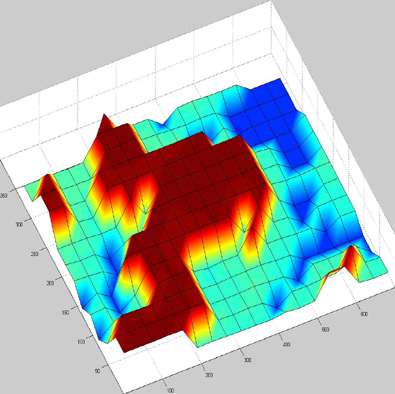
\includegraphics[width=2.8in]{3DMapDiff.jpg}
	\caption{An example task-difficulty map generated using vegetation coverage data with three difficulty levels.}
	\label{3DMapDiff}
	\end{minipage}
\end{tabular}
\end{figure}

When using a UAV to support WiSAR operations, there are two important representations of information: a \textit{probability distribution map} and a \textit{task-difficulty map}. The probability distribution map encodes information about the likely location of the missing person and is illustrated in Figure~\ref{3DMapDist}. In the figure, high values correspond to areas with high probability. The task-difficulty map encodes information about how likely it is for a searcher to detect the missing person if they were in a particular location. Figure~\ref{3DMapDiff} illustrates a task-difficulty map with high values arising from areas with, for example, dense vegetation or low visibility, indicating that likely detection is low in that area. From a Bayesian perspective, the probability distribution map encodes prior and posterior beliefs, and the task-difficulty map encodes (one minus) the likelihood of detection. Both maps are needed for effective resource allocation and task prioritization. Throughout the operation, domain experts can process information only available to them or not comprehensible by autonomous components and then incorporate such information into the \textit{probability distribution map} and the \textit{task-difficulty map} at different hierarchy, thus manage autonomy by influencing the behavior of the autonomous components through information management. 

These two maps can be created systematically using statistical models at the strategic scale by using general trends from  reliable sources. They can be easily modified by users at the between-episodes scale to incorporate additional case-specific information. They can then be used to facilitate resource allocation and UAV path planning at the within-episode scale. 

%\begin{table}
%\centering
%		\begin{tabular}{|l|c|c|}
%			\hline
%				& \multirow{2}{*}{\textbf{Probability Distribution Map}} & \multirow{2}{*}{\textbf{Task-Difficulty Map}}  \\
%				& & \\
%			\hline
%				\multirow{2}{*}{\textbf{Strategic}} & \textbf{TBMod} for map creation &  \\
%				& \textbf{ParamMod} for info management & \\
%			\hline
%				\multirow{2}{*}{\textbf{Between-Episodes}} & \textbf{DistMod} for map update &  \textbf{DiffMod} for map update \\
%				& and info management & and info management \\
%			\hline
%				\multirow{3}{*}{\textbf{Within-Episode}} & Extending algorithms to support & Extending algorithms to support\\
%				& real-time feedback &  partial detection \\ \cline{2-3}
%				& \multicolumn{2}{|c|}{\textbf{SlideMod} for info management} \\
%			\hline
%		\end{tabular}
%	\caption{Components of proposed work}	
%	\label{components}
%\end{table}

\begin{figure}
\centering
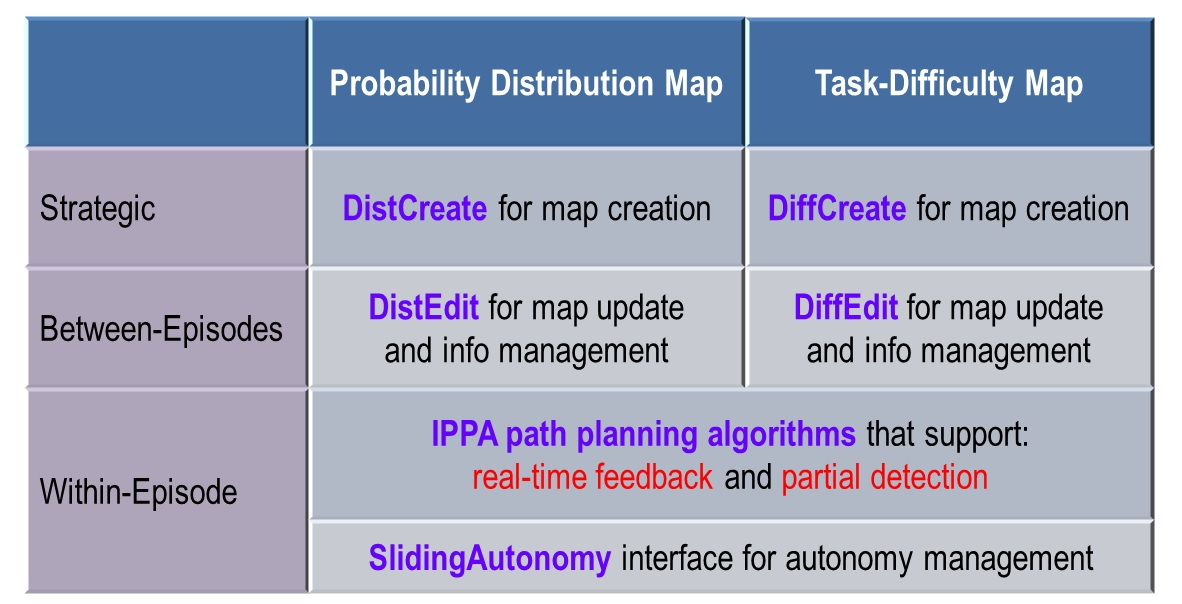
\includegraphics[width=6in]{ProjectComponents.JPG}
\caption{Autonomous components and autonomy management tools of the dissertation work at each scale/hierarchy.}
\label{ProjectComponents}
\end{figure}

Figure~\ref{ProjectComponents} lists the various components of the dissertation work as they relate to these two map representations. At the strategic scale, the \textbf{DistCreate} component uses a Bayesian model to systematically generate the probability distribution map, and the \textbf{DiffCreate} component uses Lansat data to automatically generate the task-difficulty map. At the between-episodes scale, the \textbf{DistEdit} tool and the \textbf{DiffEdit} tool enable the user to modify the probability distribution map and the task-difficulty map respectively. At the within-episode scale, we developed multiple Intelligent Path-Planning Algorithms (\textbf{IPPA}) to support real-time feedback and partial detection. We also built an information management tool, \textbf{SlidingAutonomy}, that lets the user prioritize search regions and manage the amount of autonomy desired.

All the autonomous components and autnomy management tools were designed following autonomy integration guidelines we defined in~\cite{Lin2010Supporting} (Chapter~\ref{chap:AAAI2010} of the dissertation). Figure~\ref{challenges} lists the challenges along two dimensions: \textit{attributes of an intelligent system} (capability, information management, performance evaluation) and \textit{scale} (individual, collaborative, distributed). Specifically, all the autonomous components we designed allow interactivity through the \textit{probability distribution map} and the \textit{task-difficulty map}, which enables the human agent to manage the behavior of autonomy. Additionally, the \textbf{SlidingAutonomy} management tool lets the human agent interact and manage path planning autonomy through (temporal) time allocation and (spatial) constraints (Chapter~\ref{chap:JHRI2014} of the dissertation). Chapter~\ref{chap:AAAI2010} also describe in detail how the UAV path planning problem we are solving fits in the overall intelligent system of using UAVs to support Wilderness Search and Rescue. 

%===================================================
\subsection{At the Strategic Scale}

At the strategic scale, a probability distribution map and a task-difficulty map can be created systematically.

We established in~\cite{Lin2010Bayesian} (Chapter~\ref{chap:AAAI2010} of the dissertation) a Bayesian model (\textbf{DistCreate}) that can generate the probability distribution map systematically using three types of terrain features (topography, vegetation, and elevation) and past human behavior data. Searchers first specify transitional probabilities (Beta distributions) between two terrain features as inputs. Then the model produces the prior/posterior~\cite{Russell2009Artificial} predictive probability distribution(s), which can be used to allocate resources and plan UAV paths. Figure~\ref{3DMapDist} shows an example posterior predictive probability distribution map generated by \textbf{DistCreate}. The user can influence the model-generated probability distribution by managing two types of information: \textit{model parameters} and \textit{dataset}. 

We represent the probability distribution map in discretized form using a hexagonal tessellation of the search region. We use Monte Carlo methods to encode changes in the map, so \textit{model parameters} include the users prior belief of the transition probabilities (probability of a missing person moving from one hexagonal cell to a neighbor). Transition probabilities are easily interpreted by search experts, but algorithm parameters are not. 

Although the term ``dataset'' can broadly include many sources of data, here we refer to GPS track logs of past human behavior. The user can choose whether or not to use past human behavior data. If the user chooses not to use past human behavior dataset, the \textbf{DistCreate} model will output the prior predictive distribution (prediction based only on the model parameters); otherwise, the model will output the posterior predictive distribution (prediction also based on past observations). The user can also choose what subset of the dataset to use, filtering past human behavior data by categories such as season of the year, region, or missing person profile. The user's choice will indirectly affect the probability distribution map generated by the Bayesian model.

The \textbf{DistCreate} component at this scale can download terrain vegetation coverage Lansat data directly from the USGS satelite image servers in real time when provided with GPS coordinates. Then it generates a task-difficulty map based on the type of vegetation in the specified region using a lookup table. For example, grassland is categorized as sparse vegetation and marked as easy detection area; shrub is categorized as medium vegetation and marked as medium detection area; evergreen forest is categorized as dense vegetation and marked as difficult detection area. Therefore, this component only utilizes vegetation density information when considerting the difficulty level in sensor detection. Figure~\ref{3DMapDiff} shows an example task-difficulty map generated by \textbf{DiffCreate}. It is a very simple model, and we include it for completeness. Since it is modular, it can be easily extended or replaced by more advanced detection model where factors such as ``seeability''~\cite{Morse2010UAV} (lighting condition, viewing angle, etc.) and video observer congnitive workload can be incorporated.

%===================================================
\subsection{At the Between-Episodes Scale}

At the between-episodes scale, a searcher might have additional case-specific information (e.g, past experience, knowledge of the search area or weather conditions, or the profile of the missing person) and would like to modify the general plan produced at the strategic scale. Moreover, as search progresses, the search plan should change due to newly found evidence (or the lack of it) from either the ground searchers or previous UAV flights. We developed two autonomy management tools at this scale that allow the user to manage two types of information: \textit{areas of focus} and \textit{task difficulty}. Chapter~\ref{chap:MapEdit} explains how these two tools work in detail.

\begin{figure}
\centering
\begin{tabular}{cc}
	\begin{minipage}{0.45\textwidth}
	\centering
	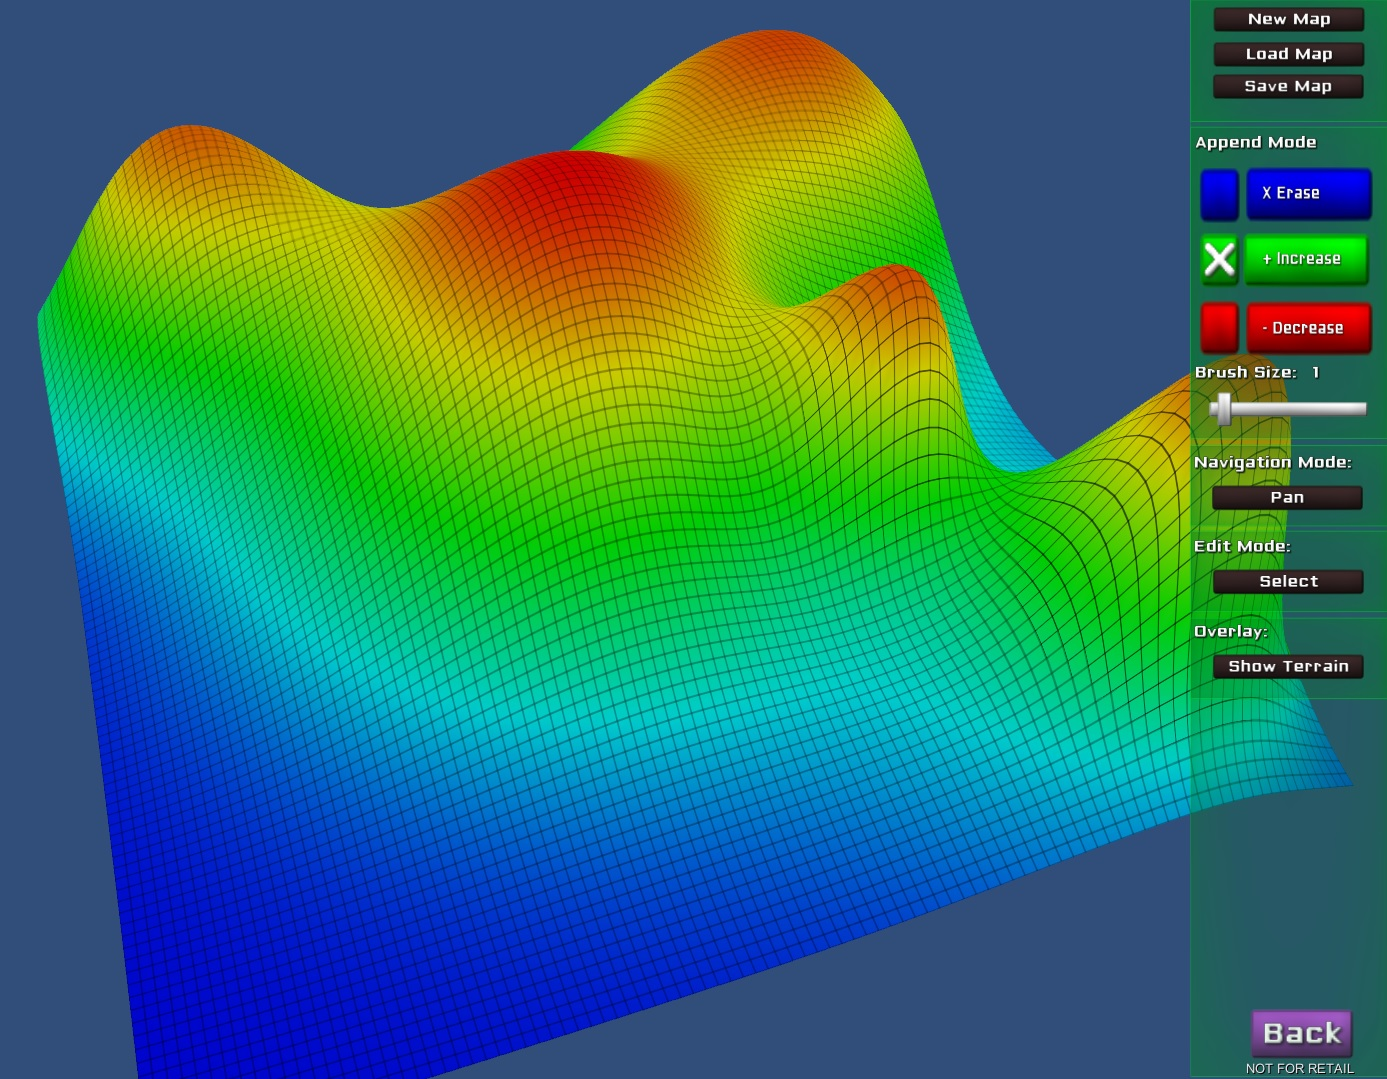
\includegraphics[width=2.8in]{DistEditExample.jpg}
	\caption{An example probability distribution map generated using the DistCreate tool.}
	\label{DistEditExample}
	\end{minipage}
&
	\begin{minipage}{0.45\textwidth}
	\centering
	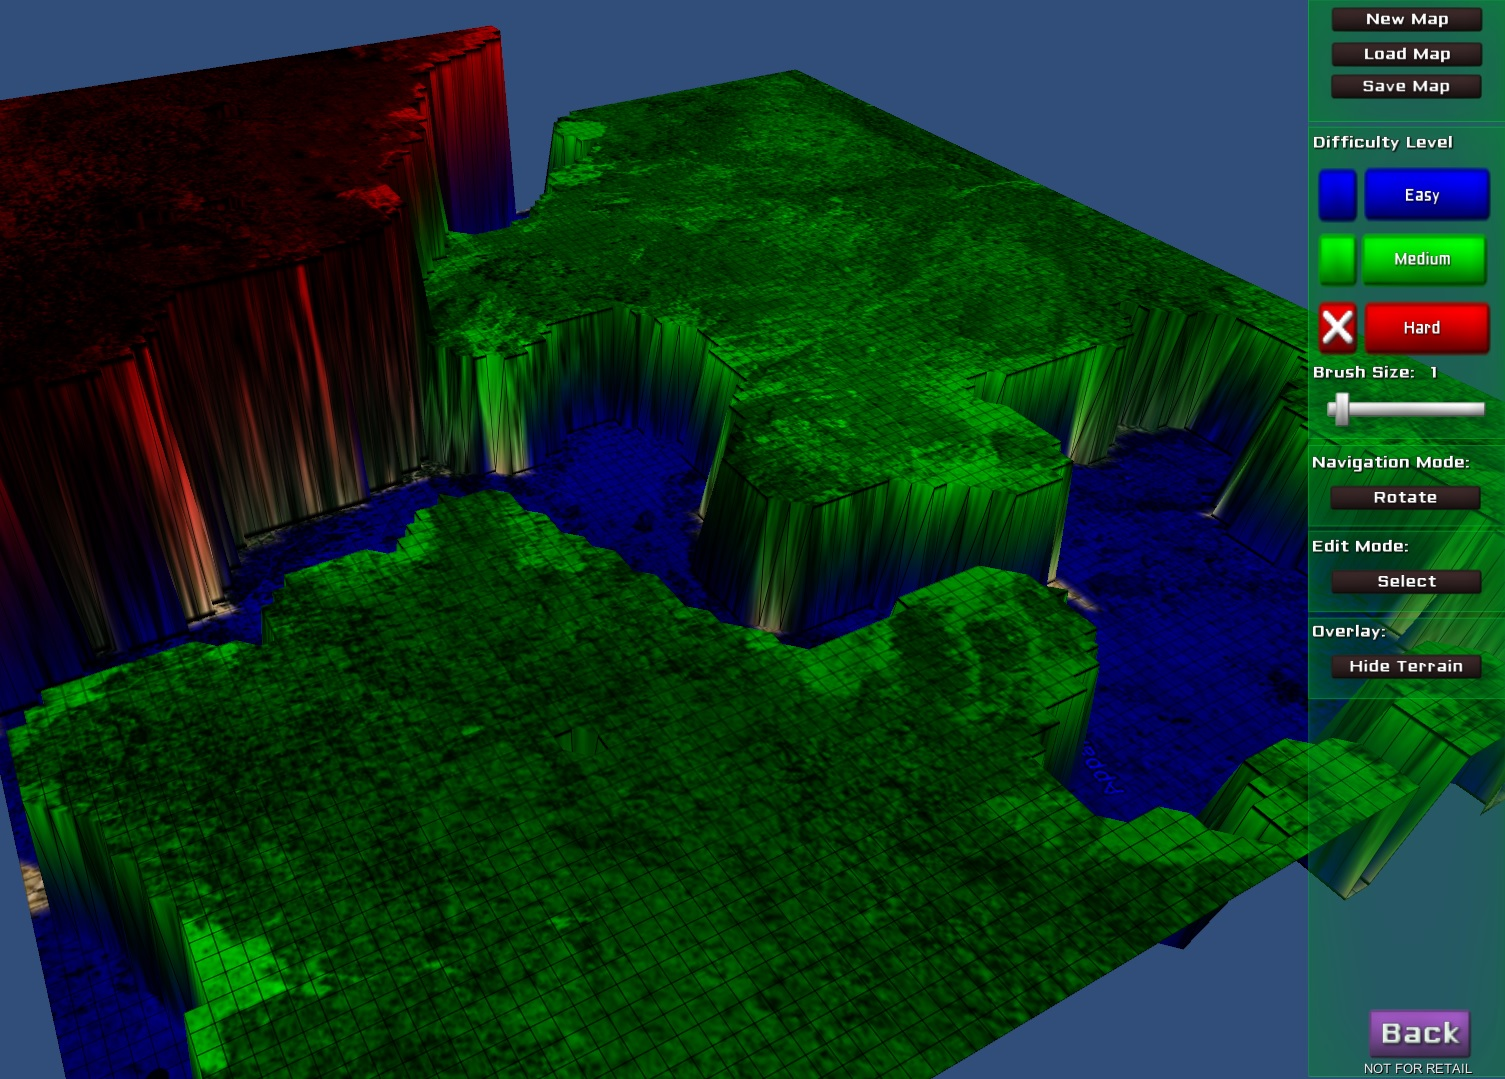
\includegraphics[width=2.8in]{DiffEditExample.jpg}
	\caption{An example task-difficulty map generated using the DiffCreate tool with satelite image of the search region overlayed on top.}
	\label{DiffEditExample}
	\end{minipage}
\end{tabular}
\end{figure}

Searchers can use the \textbf{DistEdit} tool to modify a probability distribution map and use the \textbf{DiffEdit} tool to modify a task-difficulty map generated at the \textbf{Strategic} scale. Both tools enable the user to view maps as 3D surfaces where a color map is applied for better distinction (red means high probability area or high task-difficulty level and blue means low vise versa). The user can use mouse and finger gestures to rotate/pan/zoom the respective map and edit the shapes of the maps in 3D to incorporate information that the autonomous components are unable to interprete. The user also has the option to overlay a satelite image of the search area on top of the maps for better alignments.

In \textbf{DistEdit} the user can paint Gaussian distributions onto the probability distribution map (in the form of a 3D surface) with a paintbrush tool to specify \textit{areas of focus}. The mouse click (or finger press gesture) position determines the mean of the Gaussian distribution; brush size determines the standard deviation (with a radius equivalent to three times the standard deviation); and the duration of the click (or finger press gesture) determines the scale of the Gaussian distribution. Using this tool the user can add or subtract Gaussian components to the map to create a mixture of Gaussians. The modified probability distribution can be used later to prioritize tasks and plan UAV paths. By marking an area as a high priority area, the searchers can indirectly manipulate the UAV to search the area before other areas without the need to manually specify waypoints. Figure~\ref{DistEditExample} shows an example probability distribution map generated using the \textbf{DistEdit} tool.

In \textbf{DiffEdit} the user can specify \textit{task difficulty} by using a paintbrush tool to paint on the task-difficulty map with scribbles. The user can also use a lasso tool to specify a region of irregular shape and then mark the region with selected task-difficulty level. By marking an area as a difficult area, the user can indirectly tell the UAV to make multiple passes over these areas to search more thoroughly. Figure~\ref{DiffEditExample} shows an example task-difficulty map generated using the \textbf{DiffEdit} tool with the satelite image of the search region overlayed on top.

If the user doesn't like the probability distribution map or task-difficulty map generated at the \textbf{Strategic} scale, he or she can also use the \textbf{DistEdit} and \textbf{DiffEdit} tools to create new maps from scratch. Both tools enable the searchers to add additional information (especially the type of information autonomous components cannot interprete) to the intelligent system, relying on UAV path-planning to use the information to search more efficiently.

%===================================================
\subsection{At the Within-Episode Scale}

At the within-episode scale, given a probability distribution map marking likely places to find the missing person and a task-difficulty map indicating sensor detection probability in relationship to the spatial representation of the search area, efficient UAV flight paths need to be created quickly to support WiSAR operations. We have designed multiple path planning algorithms~\cite{Lin2009UAV,Lin2014Hierarchical} so given a starting point, (optionally) an ending point, and a desired flight duration, the Intelligent Path Planning Algorithms (IPPA) can generate flight paths that approximate the optimal path (see Figure~\ref{path} for an example) to maximize the probability of finding the missing person.

\begin{figure}
\centering
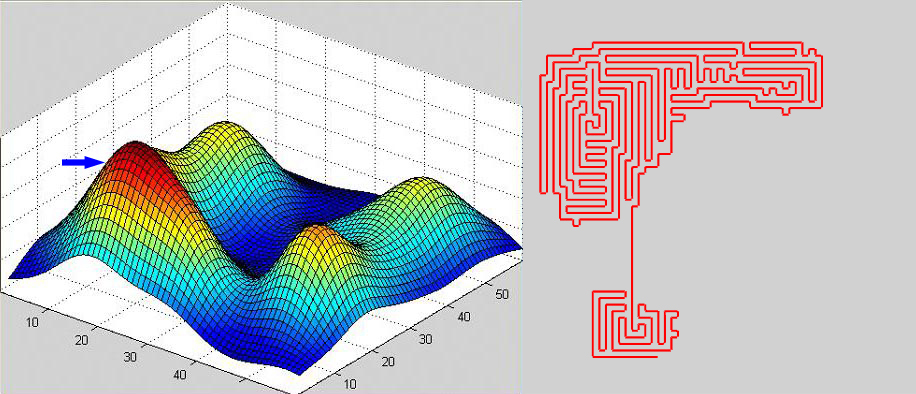
\includegraphics[width=6in]{ComplexMap.jpg}
\caption{Example UAV path generated for a complex multi-model distribution by a path planning algorithm. (The blue arrow indicates the starting point.)}
\label{path}
\end{figure}

We present in~\cite{Lin2009UAV} (Chapter~\ref{chap:IROS2009} of the dissertation) multiple intelligent path planning algorithms using Local-Hill Climbing, Potential Field, lawnmower patterns, and Evolutionary Algorithm techniques. We evaluate the performance of these algorithms against simple and complicated synthetic scenarios with the assumption of 100\% detection probability (no task-difficulty map is used). Then in~\cite{Lin2014Hierarchical} (Chapter~\ref{chap:SMCB2014} of the dissertation) we extended these algorithms to support partial detection by introducing the task-difficulty map, and also present two new (Top2 and TopN) algorithms, which utilize the \textit{Mode Goodness Ratio} heuristic we designed and enable a hierarchical search in the parameter space. We compare the performance of these algorithms against Bourgault's Algorithm~\cite{Bourgault2006Optimal} and the LHC-GW-CONV~\cite{Lin2009UAV} algorithm using three real WiSAR scenarios, and the Top2 and TopN algorithms outperformed both algorithms. To improve computation time of these algorithms, we implemented hierarchical coarse-to-fine search and hierarchical desicion making. Algorithms were also parallelized to take advantage of multi-core processor capabilities. More details can be found in Appendix~\ref{chap:hierarchical}.

When new evidence is gathered (from UAV aerial imagery or from ground searchers) while the UAV is flying, the search plan might need to be changed in real-time. At this within-episode scale, the information management tools \textbf{DistEdit} and \textbf{DiffEdit} previously proposed can still be used to update the probability distribution and the task-difficulty maps. This provides flexibility in autonomy management. Additionally, we have designed an autonomy management interface, \textbf{SlidingAutonomy}, that enables the user to prioritize search regions and manage the desired amount of the autonomous local search along two new dimensions: changing the desired flight duration (temporal control) and adding constraints (endpoints, spatial control).

The \textbf{SlidingAutonomy} tool allows a searcher to specify a starting point and (optionally) an ending point on the terrain satelite image overlay. Then, by moving a slider, the user can control how much flight time is granted, and the IPPA algorithms generate UAV paths within the local region. Beginning from the ending point of the previous flight path segment, the searcher can plan the next path segment in the next search region. This way, the searcher can specify the order of different search regions and let the algorithm determine what paths the UAV should follow at each region. By setting flight duration and adding constraints, the searcher tells the UAV information about search priorities and at the same time, indirectly manages the local path planning based on his/her own judgment of how much the UAV can be trusted to cover a given area well. This autonomy management tool gives the user the flexibility of controlling the amount of autonomy desired without the burden of creating the entire flight path manually through waypoints. Figure~\ref{SlidingAutonomy} shows an example path depicting prioritized search regions and local paths. As the user moves the slider in the \textbf{SlidingAutonomy} tool, the system provide immediate visual feedback of what local path the system generates. This way, the searcher can easily infer the causal relationship between his/her actions (changes in flight duration) and the autonomous behaviors of the system (what path is generated). 

\begin{figure}
\centering
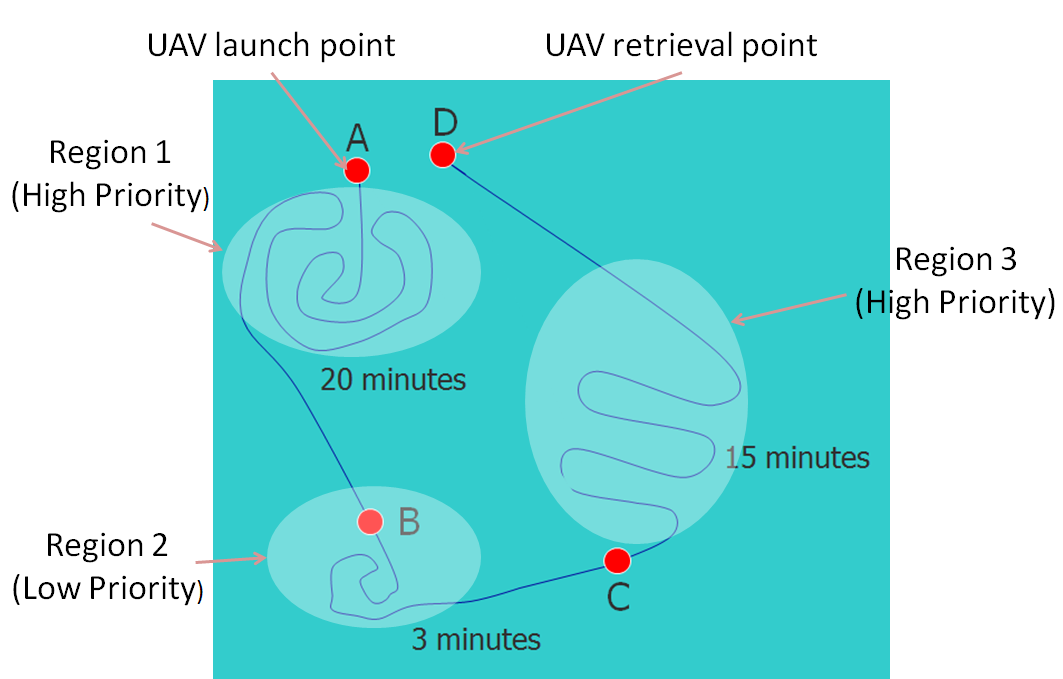
\includegraphics[width=6in]{SlidingAutonomyE.png}
\caption[An example scenario of path planning using sliding autonomy]{An example scenario of path planning using sliding autonomy: The UAV is launched at point A. Because region 1 is a high priority area, the searcher lets the UAV search for 20 minutes before arriving at point B, resulting in a longer flight path. Region 2 has low priority, so the searcher only gives the UAV 3 minutes before sending the UAV to point C, resulting in a short flight path. Region 3 is a high priority area, so the searcher gives the UAV 15 minutes. But the UAV also needs to reach Point D, the UAV retrieval point, at the end of the allocated 15 minutes. A medium length flight path is generated to meet the requirements.}
\label{SlidingAutonomy}
\end{figure}

We performed a user study to validate the usefulness of the approach. Experiment results show that the human-automation team outperforms human or automation working alone, reduces the human's cognitive workload, and improves the human experience in the human-automation interaction (Chapter~\ref{chap:JHRI2014} of the dissertation).


%=====================================================================================================
\section{Dissertation Chapters}

This dissertation consists of five papers, two of which are under review. This section gives a brief description of each chapter.

%===================================================
\subsection{Chapter Descriptions}

Chapter~\ref{chap:intro} gives an overview of our proposed autonomy management approach and provides an overall related literature review with respect to autnomy management approaches and path planning for UAV in the context of Wilderness Search and Rescue. It explains how all the components in our dissertation fit in the hierarchical structure and how they related to chapters of this dissertation.

Chapter~\ref{chap:AAAI2010} presents autonomy integration guidelines we identified (see Figure~\ref{challenges} when integrating UAV autonomies to the WiSAR system. We summarize the challenges along two dimensions: \textit{attributes of an intelligent system} (capability, information management, performance evaluation) and \textit{scale} (individual vs. group). The table was extended later (in Chapter~\ref{chap:JHRI2014}) to include a row for collaborative agents when a human agent works together with the autonomous agent. The paper emphasize on how information management is an important attribute of an intelligent system, where users assign tasks to autonomous algorithms by matching capabilities of the autonomous agents based on information fusion from the overall distributed system. It also describes in detail how the UAV path planning problem fits in the overall intelligent system of using UAVs to support Wilderness Search and Rescue.

In chatper~\ref{chap:CMOT2010} we present a Bayesian model that uses publicly available terrain features data to help model lost-person behaviors. This approach enables domain experts to encode uncertainty in their prior estimations and also makes it possible to incorporate human behavior data collected in the form of posterior distributions. It also enables the searcher to influence the probability distribution map generated by changing prior beliefs in the transitional probabilities between terrain features and by selecting what subset of past human behavior data to feed to the model.

Chapter~\ref{chap:IROS2009} explores several path planning algorithms (with and without set destination) and describe some novel techniques in solving the problem of maximizing sensor (UAV onboard video camera) coverage within a set time to support Wilderness Search and Rescue. The task-difficulty map is not used and we assume 100\% detection probability. Performance of these algorithms are compared against typical WiSAR scenarios, and experiment results show that these algorithms yield high quality solutions that approximate the optimal solution.

Chapter~\ref{chap:SMCB2014} proposes a heurisitc, \textit{Mode Goodness Ratio}, which uses a Gaussian Mixture Model to prioritize search subregions, and presents two path planning algorithms (Top2 and TopN) that utilize the heuristic and hierarchically search for effective paths through the parameter space at different levels of resolution. Performance of the new algorithms are compared against two published algorithms (Bourgault's algorithm and LHC-GW-CONV algorithm) in simulated searches with three real search and rescue scenarios where both the probability distribution map and the task-difficulty map are used. Results show that the new algorithms outperform existing algorithms significantly when partial detection is considered, and can yield efficient paths that yield payoffs near the optimal. 

Chapter~\ref{chap:JHRI2014} extends the autonomy integration guidelines we identified in Chapter~\ref{chap:AAAI2010} to include collaborative agents when a human agent works together with the autonomous agent. It proposes two additional dimensions for autonomy management: time allocation (temporal) and constraints (spatial), and presents a new autonomy management approach named \textbf{Sliding Autonomy} where the human agent in the human-automation team can assign different flight duration to the path planning algorithms to plan path segments and use endpoints to manage search region priorities. A user study was performed to validate the usefulness of the approach. Experiment results show that the human-automation team outperforms human or automation working alone, reduces the human's cognitive workload, and improves the human experience in the human-automation interaction.

Chatper~\ref{chap:MapEdit}



In chapter~\ref{chap:Conclusions} concludes findings of the dissertation work and 


%===================================================
\subsection{Publications List}

We list all the citations for each chapter in the order in which they appear.

1. Jie Long, Cory Reimschussel, Ontario Britton, Anthony Hall, and Michael Jones. Performance Capture for Natural Tree Motions in the Wind. Motion in Games , MIG, 2010. 

2. Jie Long, Bryce Porter, Michael Jones. Motion Capture of Rope, not yet published.


